\documentclass[a4paper,11pt,titlepage]{article}

\usepackage[czech, slovak]{babel}
\usepackage[IL2]{fontenc}
\usepackage[utf8]{inputenc}
\usepackage{times}
\usepackage[ruled,czech,linesnumbered,longend,noline]{algorithm2e}
\usepackage{graphics}
\usepackage[unicode]{hyperref}
\usepackage{graphicx}
\usepackage{amsmath}

\makeatletter
\def\@seccntformat#1{%
  \expandafter\ifx\csname c@#1\endcsname\c@section\else
  \csname the#1\endcsname\quad
  \fi}
\makeatother

\usepackage[left=20mm, text={170mm, 240mm}, top=30mm]{geometry}

\begin{document}

\begin{titlepage}

\begin{center}
    {\Huge\textsc{Vysoké učení technické v~Brně}}\\
        \medskip
    {\huge\textsc{Fakulta informačních technologií}}\\
    \vspace{\stretch{0.382}}
    {\LARGE 	Elektronika pro informační technologie}\\
        \medskip
    {\Huge Semestrální projekt}\\
    \vspace{\stretch{0.618}}
\end{center}

{\LARGE \today \hfill
Róbert Ďurovič [xdurov01]}

\end{titlepage}

\section{Príklad č. 1 - varianta D}

Stanovte napětí $U_{R_1}$ a proud $I_{R_1}$. Použijte metodu postupného zjednodušování obvodu.

\vspace{5mm}

\begin{tabular}{ |c|c|c|c|c|c|c|c|c|c| } \hline
    $U_1$ [V] & $U_2$ [V] & $R_1$ [$\Omega$] & $R_2$ [$\Omega$] & $R_3$ [$\Omega$] & $R_4$ [$\Omega$] & $R_5$ [$\Omega$] & $R_6$ [$\Omega$] & $R_7$ [$\Omega$] & $R_8$ [$\Omega$]\\ \hline
    105 & 85 & 420 & 980 & 330 & 280 & 310 & 710 & 240 & 200 \\ \hline
\end{tabular}

\vspace{5mm}

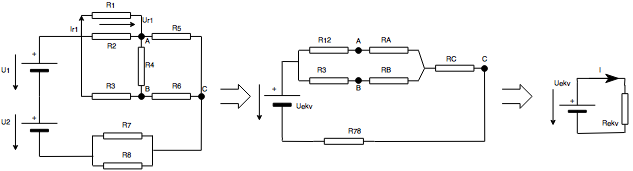
\includegraphics[scale=0.7]{dia.png}

\vspace{5mm}

Vypočítame napätie pre obvod $U_{EKV}$:
\[U_{EKV} = U_1 + U_2 = 190 V\]

\vspace{5mm}

Vypočítame odpor paralelne zapojených rezistorov $R_7$ a $R_8$:
\[R_{78} = \frac{R_7 \cdot R_8}{R_7 + R_8} = \frac{48000}{440} = 109,090909 \Omega\]

\vspace{5mm}

Vypočítame odpor paralelne zapojených rezistorov $R_1$ a $R_2$:
\[
R_{12} = \frac{R_1 \cdot R_2}{R_1 + R_2} = \frac{411600}{1400} = 294 \Omega
\]

\vspace{5mm}

Vypočítame odpor rezistorov zapojených do hviezdy:
\begin{align*}
R_A &= \frac{R_4 \cdot R_5}{R_4 + R_5 + R_6} = \frac{280 \cdot 314}{280 + 310 + 710} = \frac{86800}{1300} = 66,76923 \Omega \\[10pt]
R_B &= \frac{R_4 \cdot R_6}{R_4 + R_5 + R_6} = \frac{280 \cdot 710}{1300} = 152,92307 \Omega \\[10pt]
R_C &= \frac{R_5 \cdot R_6}{R_4 + R_5 + R_6} = \frac{310 \cdot 710}{1300} = 169,30769 \Omega 
\end{align*}

\vspace{5mm}

Vypočítame celkový odpor $R_{EKV}$:
\begin{align*}
R_{EKV} &= R_C + \frac{(R_A + R_{12}) \cdot (R_B + R_3)}{(R_A + R_{12}) + (R_B + R_3)} + R_{78} \\[10pt]
R_{EKV} &= 169,30769 + \frac{360,76923 \cdot 482,92307}{360,76923 + 482,92307} + 109,090909 \\[10pt]
R_{EKV} &= 169,30769 + 375,80925 + 109,090909 \\[10pt]
R_{EKV} &= 484,90016 \Omega 
\end{align*}

\vspace{5mm}

Vypočítame prúd $I$:
\[
I = \frac{U_{EKV}}{R_{EKV}} = \frac{190}{484,90016} = 0,39183A
\]

\vspace{5mm}

\begin{align*}
U_R &= \frac{(R_A + R_{12}) \cdot (R_B + R_3)}{(R_A + R_{12})} \cdot I \\[10pt]
U_R &= 206,50169 \cdot 0,39183 \\[10pt]
U_R &= 80,913509V
\end{align*}

\vspace{5mm}

\begin{align*}
I_R &= \frac{U_R}{(R_A + R_{12})} \\[10pt]
I_R &= 0,2242805A
\end{align*}

\vspace{5mm}

Vypočítame napätie $U_{R_1}$
\begin{align*}
U_{R_1} &= U_{R_{12}} = R_{12} \cdot I_R \\[10pt]
U_{R_1} &= 65,9385V
\end{align*}

\vspace{5mm}

Vypočítame prúd $I_{R_1}$
\begin{align*}
I_{R_1} &= \frac{U_{R_1}}{R_1} \\[10pt]
I_{R_1} &= \frac{65,9385}{420} \\[10pt]
I_{R_1} &= 0,1570A
\end{align*}

\newpage

\section{Príklad č. 2 - varianta F}

Stanovte napětí $U_{R_3}$ a proud $I_{R_3}$. Použijte metodu Théveninovy věty.

\vspace{5mm}

\begin{tabular}{ |c|c|c|c|c|c| } \hline
    $U_1$ [V] & $U_2$ [V] & $R_1$ [$\Omega$] & $R_2$ [$\Omega$] & $R_3$ [$\Omega$] & $R_4$ [$\Omega$]  \\ \hline
    130 & 180 & 300 & 600 & 195 & 650 \\ \hline
\end{tabular}

\vspace{5mm}

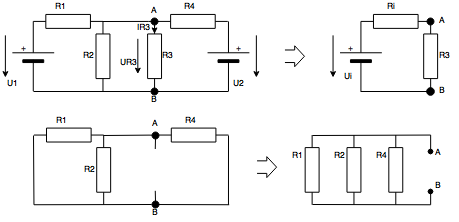
\includegraphics[scale=0.85]{diag.png}

\vspace{5mm}

Vzorec pre výpočet $R_i$:
\[R_{124} = R_i = R_1 \parallel R_2 \parallel R_4 = \frac{1}{\frac{1}{R_1} + \frac{1}{R_2} + \frac{1}{R_4}}\]

\vspace{5mm}

Vzorec pre výpočet $U_i$:
\[U_i = R_{124} \cdot I_{12}\]

\vspace{5mm}

Vzorec pre výpočet $I_{R_3}$:
\[I_{R_3} = \frac{U_i}{R_i + R_3}\]

\vspace{5mm}

Vzorec pre výpočet $U_{R_3}$:
\[U_{R_3} = I_{R_3} \cdot R_3\]

\vspace{5mm}

Výpočet $I_1$:
\[I_1 = \frac{U_1}{R_1} = \frac{130}{350} = 0,3714A\]

\vspace{5mm}

Výpočet $I_2$:
\[I_2 = \frac{U_2}{R_4} = \frac{180}{650} = 0,2769A\]

\vspace{5mm}

Výpočet $I_{12}$:
\[I_{12} = I_1 + I_2 = 0,6484A\]

\vspace{5mm}

Dosadíme do vzorca pre $R_i$:
\[R_i = \frac{1}{\frac{1}{350} + \frac{1}{600} + \frac{1}{650}} = 164,9547 \Omega\]

\vspace{5mm}

Dosadíme do vzorca pre $U_i$:
\[U_i = 164,9547 \cdot 0,6484 = 106,9486V\]

\vspace{5mm}

Dosadíme do vzorca pre $I_{R_3}$:
\[I_{R_3} = \frac{106,9486}{164,9547 + 195} = 0,2971A\]

\vspace{5mm}

Dosadíme do vzorca pre $U_{R_3}$:
\[U_{R_3} = 0,2971 \cdot 195 = 57,9378V\]

\newpage

\section{Príklad č. 3 - varianta B}

Stanovte napětí $U_{R_5}$ a proud $I_{R_5}$. Použijte metodu uzlových napětí ($U_A$, $U_B$, $U_C$).

\vspace{5mm}

\begin{tabular}{ |c|c|c|c|c|c|c|c| } \hline
    $U$ [V] & $I_1$ [A] & $I_2$ [A] & $R_1$ [$\Omega$] & $R_2$ [$\Omega$] & $R_3$ [$\Omega$] & $R_4$ [$\Omega$] & $R_5$ [$\Omega$] \\ \hline
    150 & 0,7 & 0,8 & 49 & 45 & 61 & 34 & 34 \\ \hline
\end{tabular}

\vspace{5mm}

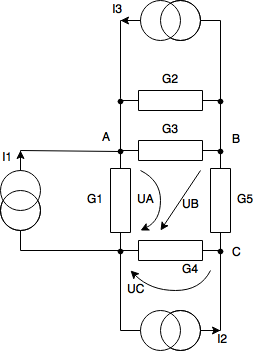
\includegraphics[scale=0.5]{diagr.png}

\vspace{5mm}

Vypočítame prúd $I$:
\[I = \frac{U}{R_2} = \frac{150}{45} = 3,3333A\]

\vspace{5mm}

Zostavíme maticu:
$$
\begin{bmatrix}
  \; {G_1 + G_2 + G_3} & {-G_2 - G_3} & {0} \; \\
  \; {-G_2 - G_3} & {G_2 + G_3 + G_5} & {-G_5} \; \\
  \; {0} & {-G_5} & {G_4 + G_5} \;
\end{bmatrix} 
\cdot
\begin{bmatrix}
  \; U_A \; \\
  \; U_B \; \\
  \; U_C \;
\end{bmatrix} =
\begin{bmatrix}
  \; I + I_1 \; \\
  \; -I \; \\
  \; I_2 \;
\end{bmatrix} 
$$

\vspace{5mm}

Upravíme:
$$
\begin{bmatrix}
  \; U_A \; \\
  \; U_B \; \\
  \; U_C \;
\end{bmatrix} =
\begin{bmatrix}
  \; {0,0590} & {-0,03862} & {0} \; \\
  \; {-0,03862} & {0,06803} & {-0,02941} \; \\
  \; {0} & {-0,02941} & {0,05882} \;
\end{bmatrix}^{-1} 
\cdot
\begin{bmatrix}
  \; 4,0333 \; \\
  \; -3,3333 \; \\
  \; 0,8 \;
\end{bmatrix} 
$$

\vspace{5mm}

Dopočítame $U_A$, $U_B$, $U_C$:
\begin{align*}
U_A &= 61,46528686V \\
U_B &= -10,349876543V \\
U_C &= 8,350617284V
\end{align*}

\vspace{5mm}

Vypočítame $U_{R_5}$
\[U_{R_5} = U_C - U_B = 8,3506 - (-10,4988) = 18,8494V\]

\vspace{5mm}

Vypočítame $I_{R5}$:
\[I_{R_5} = \frac{U_{R_5}}{R_5} = \frac{18,8494}{34} = 0,5544A\]

\newpage

\section{Príklad č. 4 - varianta D}

Pro napájecí napětí platí: $u_1 = U_1 \cdot \sin(2 \pi ft), u_2 = U_2 \cdot \sin(2 \pi ft).$ 
Ve vztahu pro napětí \\ $u_{C_1} = U_{C1} \cdot \sin(2 \pi ft +
\varphi C_1)$ určete $\mid U_{C_1} \mid$ a $\varphi C_1$. Použijte metodu smyčkových proudů.
\vspace{5mm}

\begin{tabular}{ |c|c|c|c|c|c|c|c|c|c| } \hline
    $U_1$ [V] & $U_2$ [V] & $R_1$ [$\Omega$] & $R_2$ [$\Omega$] & $R_3$ [$\Omega$] & $R_4$ [$\Omega$] & $R_5$ [$\Omega$] & $R_6$ [$\Omega$] & $R_7$ [$\Omega$] & $R_8$ [$\Omega$]\\ \hline
    105 & 85 & 420 & 980 & 330 & 280 & 310 & 710 & 240 & 200 \\ \hline
\end{tabular}

\vspace{5mm}

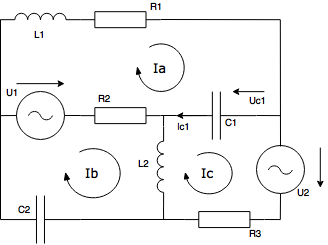
\includegraphics[scale=0.7]{diagra.png}

\vspace{5mm}

\[\omega = 2 \pi f = 533,8 rad/s\]

\begin{align*}
X_{C_1} &= \frac{-1}{j\omega C_1} = \frac{-1}{0,112098} = -8,920765759j \\[10pt]
X_{C_2} &= \frac{-1}{j\omega C_2} = \frac{-1}{0,040035} = -24,97814412j \\[20pt]
X_{L_1} &= j\omega L_1 = 96,084j \\[10pt]
X_{L_2} &= j\omega L_2 = 48,042j
\end{align*}

\vspace{5mm}

Zostavíme sústavu rovníc:
\begin{align*}
I_A &: \quad (X_{L_1} + R_1) \cdot I_A + X_{C_1} \cdot (I_A - I_C) + R_2 \cdot (I_A - I_B) = U_1 \\
I_B &: \quad X_{C_2} \cdot I_B + R_2 \cdot (I_B - I_A) + X_{L_2} \cdot (I_B - I_C) = -U_1 \\
I_C &: \quad R_3 \cdot I_C + X_{L_2} \cdot (I_C - I_B) + X_{C_1} \cdot (I_C - I_A) = -U_2
\end{align*}

\vspace{5mm}

Vypočítame $I_{c_1}$ a $U_{c_1}$:
\[I_{c_1} = I_A - I_C = 1,41A\]

\[U_{c_1} = X_{C_1} \cdot I_{c_1}\]
\[\mid U_{c_1} \mid = \sqrt{{R_e}^2 + {I_m}^2} = 13,15V\]

\vspace{5mm}

Zistíme fázový posun $\varphi_{c_1}$:
\[\varphi_{c_1} = arctan \frac{I_m}{R_e}\]

\vspace{5mm}

Prevedieme do sptávneho kvadrantu:
\[\varphi_{c_1} + 180^{\circ}\]


\newpage

\section{Príklad č. 5 - varianta F}

Sestavte diferenciální rovnici popisující chování obvodu na obrázku, dále ji upravte dosazením hodnot parametrů. Vypočítejte analytické řešení $U_c$ = $f(t)$. Proveďte kontrolu výpočtu dosazením do sestavené diferenciální rovnice.

\vspace{5mm}

\begin{tabular}{ |c|c|c|c| } \hline
    $U$ [V] & $C$ [F] & $R$ [$\Omega$] & $u_c$(0) [V]  \\ \hline
    45 & 30 & 15 & 4 \\ \hline
\end{tabular}

\vspace{5mm}

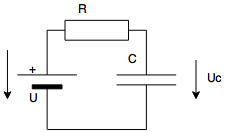
\includegraphics[scale=0.7]{diagram.png}

\vspace{5mm}

Axióm:
\[U'_c = \frac{1}{C} \cdot I_c\]

\vspace{5mm}

Pre celkové napätie platí:
\[U_R + u_c - U = 0 \]
\[U = R \cdot I + U_c \] 
\[I_c = \frac{U - U_c}{R} \]

\vspace{5mm}

Dosadenie zadanej hodnoty:
\[U'_c = \frac{1}{C} \cdot \frac{U - U_c}{R} = \frac{1 \cdot (45 - U_c)}{450} \]

\vspace{5mm}

Charakteristická rovnica:
\[C \cdot R \cdot U_c' + U_c = U\]
\[30 \cdot 15 \cdot U_c' + U_c = 45\]
\[ 450 \cdot U_c' + U_c = 45 \hspace{5mm} u_c(0) = 4\]
\[450\lambda + 1 = 0 \hspace{5mm} \lambda = -0,002222\]

\vspace{5mm}

Očakávané riešenie:
\[U_c(t) = C(t) \cdot e^{\lambda t} = C(t) \cdot e^{-0,002222t}\]
\[U_c'(t) = C'(t) \cdot e^{\lambda t} + C(t) \cdot \lambda \cdot e^{\lambda t}\]

\vspace{5mm}

Dosadenie do charakteristickej rovnice:
\[450(C'(t) \cdot e^{\lambda t} + C(t) \cdot \lambda \cdot e^{\lambda t}) - 45\]
\[450 \cdot C'(t) \cdot e^{\lambda t} = 45\]
\[C'(t) \cdot e^{\lambda t} = 0,1\]
\[C'(t) = \frac{0,1}{e^{\lambda t}} = \frac{0,1}{e^{-0,002222t}} = 0,1^{0,002222t}\]

\vspace{5mm}

Integrácia:
\[C(t) = 0,1 \cdot \frac{1}{0,002222} \cdot e^{-0,002222t} = 45 \cdot e^{-0,002222t} + q\]

\vspace{5mm}

Dosadenie do očakávaného riešenia:
\[U_c(t) = (45 \cdot e^{0,002222t} + q) \cdot e^{-0,002222t} = 6 + q \cdot e^{-0,0022t}\]

\vspace{5mm}

Nájdenie $q$:
\[U_c(0) = 4\]
\[4 = 45 + q \cdot e^0\]
\[q = -41\]
\[U_c = 45 - 41 \cdot e^{-0,002222t}\]

\vspace{5mm}

Skúška:
\[450 \cdot U_c' + U_c = 45\]
\[0 + 4 \cdot e^{-0,002222t} + 45 - 4 \cdot e^{-0,002222t} = 45\]
\[45 = 45\]

Diferenciálna rovnica je správna.

\newpage

\section{Súhrn výsledkov}

\begin{tabular}{ |c|c|c| } \hline
    úloha & varianta & výsledky \\ \hline
    1 & D & $I_{R_1}$ = 0,1570A \quad $U_{R_1}$ = 65,9385V \\ \hline
    2 & F & $I_{R_3}$ = 0,2971A \quad $U_{R_3}$ = 57,9378V\\ \hline
    3 & B & $I_{R_5}$ = 0,5544A \quad $U_{R_5}$ = 18,8494V\\ \hline
    4 & D & $U_{c_1}$ = 13,15V \\ \hline
    5 & F & \\ \hline
\end{tabular}

\end{document}
